\documentclass[EEEE]{KGCOEReport}

\usepackage[backend=biber]{biblatex}
\usepackage{graphicx}
\usepackage{newtxtext, newtxmath}
\usepackage{csquotes}
\usepackage{parskip}
\usepackage{karnaugh-map}
\usepackage{amsmath}
\usepackage{circuitikz}
\usepackage{hyperref}
\usepackage{float}
\usepackage{pdfpages}
\usepackage{pgfplots, pgfplotstable}

\graphicspath{./assets/}
\addbibresource{./assets/bib.bib}

\newcommand{\classCode}{EEEE 281}
\newcommand{\className}{Circuits 1}

\newcommand{\name}{Aden Perry}
% \newcommand{\partnerName}{PARTNER}

\newcommand{\LabSectionNum}{L7}

\newcommand{\TAs}{Sol Holston}
\newcommand{\exerciseNumber}{4}
\newcommand{\exerciseDescription}{Op-amps 1}

\newcommand{\dateDone}{2026-04-07}
\newcommand{\dateSubmitted}{2026-04-14}

\pgfplotsset{compat=1.18}

\begin{document}

\maketitle

\section*{Abstract}

The purpose of this exercise was to examine inverting and non-inverting
operation amplifiers and determine the gain. Two circuits, each containing one
configuration of the op-amp, were analyzed. Hand calculations were performed to
find the required resistance values to achieve a gain of -4.7 and +3.2,
respectively. Both circuits were simulated with the calculated resistances
using LTspice to confirm correctness. Transient simulations were performed on
each circuit using a sinusoidal source. Trace cursors were used to calculate
the gain ratio of each circuit. Each circuit was implemented in hardware using
a function generator as a source. Gain ratios were measured using an
oscilliscope. The simulated and measured gain ratios were similar to -4.7 and
+3.2, respectively; the exercise was successful.

\section{Introduction and Theory}

The objective of this laboratory was to calculate resistances required for a
given gain ratio; to apply varying voltages to inverting and non-inverting
op-amp circuits; and to measure the gain of inverting and non-inverting
op-amps.

\subsection{Theory: Circuit Investigated}

An inverting op-amp circuit is given in Figure \ref{fig:opinv}.

\begin{figure}[H]
	\center
	\includegraphics[width=0.5\textwidth]{figures/circuit1.pdf}
	\caption{Inverting Circuit}
	\label{fig:opinv}
\end{figure}

A sinusoidal voltage source is connected to a kilo-ohm resistor and then to
the inverting terminal of an operational amplifier. The inverting terminal is
also connected to a resistor of unknown resistance, $R_f$, and then to the
output terminal. The non-inverting terminal is attached to ground. Output
voltages will be clipped to $\pm$5 V.

By inspection, Equation \ref{eqn:e1} is found:

\begin{align}
	- \frac{V_{in}}{R_1} & =  \frac{V_{out}}{R_f}    \notag \\
	- \frac{R_f}{R_1}    & =  \frac{V_{out}}{V_{in}}
	\label{eqn:e1}
\end{align}

Using Equation \ref{eqn:e1}, the value of $R_f$ required to obtain a gain ratio
of -4.7, assuming a resistance $R_1$ of 1 kilo-ohm can be obtained. The
derivation is given in Equation \ref{eqn:e2}:

\begin{align}
	-\frac{R_f}{R_1}               & = \frac{V_{out}}{V_{in}} \notag \\
	-\frac{R_f}{\left(1000\right)} & = \left(-4.7\right)     \notag  \\
	R_f                            & = 4700
	\label{eqn:e2}
\end{align}

Thus, the resistance $R_f$ for a gain ratio of -4.7 is found to be 4.7
kilo-ohms.

A non-inverting op-amp circuit is given in Figure \ref{fig:opnon}.

\begin{figure}[H]
	\center
	\includegraphics[width=0.5\textwidth]{figures/circuit2.pdf}
	\caption{Non-Inverting Circuit}
	\label{fig:opnon}
\end{figure}

The non-inverting op-amp circuit is much the same as the circuit given in
Figure \ref{fig:opinv}, except the voltage source is moved to the non-inverting
terminal of the op-amp.

By inspection, Equation \ref{eqn:e3} is found:

\begin{align}
	\frac{V_{in}}{R_1}     & = \frac{V_{out} - V_{in}}{R_f} \notag                   \\
	\frac{R_f}{R_1}        & = \frac{V_{out}}{V_{in}} - \frac{V_{in}}{V_{in}} \notag \\
	\frac{V_{out}}{V_{in}} & = \frac{R_f}{R_1} + 1
	\label{eqn:e3}
\end{align}

Using Equation \ref{eqn:e3}, the value of $R_f$ required to obtain a gain ratio
of 3.2, assuming a resistance $R_1$ of 1 kilo-ohm can be obtained. The
derivation is given in Equation \ref{eqn:e4}:

\begin{align}
	\frac{V_{out}}{V_{in}} & = \frac{R_f}{R_1} + 1  \notag              \\
	\left(3.2\right)       & = \frac{R_f}{\left(1000\right)} + 1 \notag \\
	R_f                    & = 2200
	\label{eqn:e4}
\end{align}

Thus, the resistance $R_f$ for a gain ratio of 3.2 is found to be 2.2
kilo-ohms.

\subsection{Theory: LTspice Simulation}

The inverting circuit was simulated using LTSpice. The LTSpice circuit
schematic is shown in figure \ref{fig:lts-c1}.

\begin{figure}[H]
	\center
	
\includegraphics[width=\textwidth]{./assets/c1.png}
	\caption{Circuit 1 in LTspice}
	\label{fig:lts-c1}
\end{figure}

The schematic given by Figure \ref{fig:lts-c1} was used to run a transient
simulation, the results of which are given in Figure \ref{fig:lts-c1-trace}.

\begin{figure}[H]
	\center
	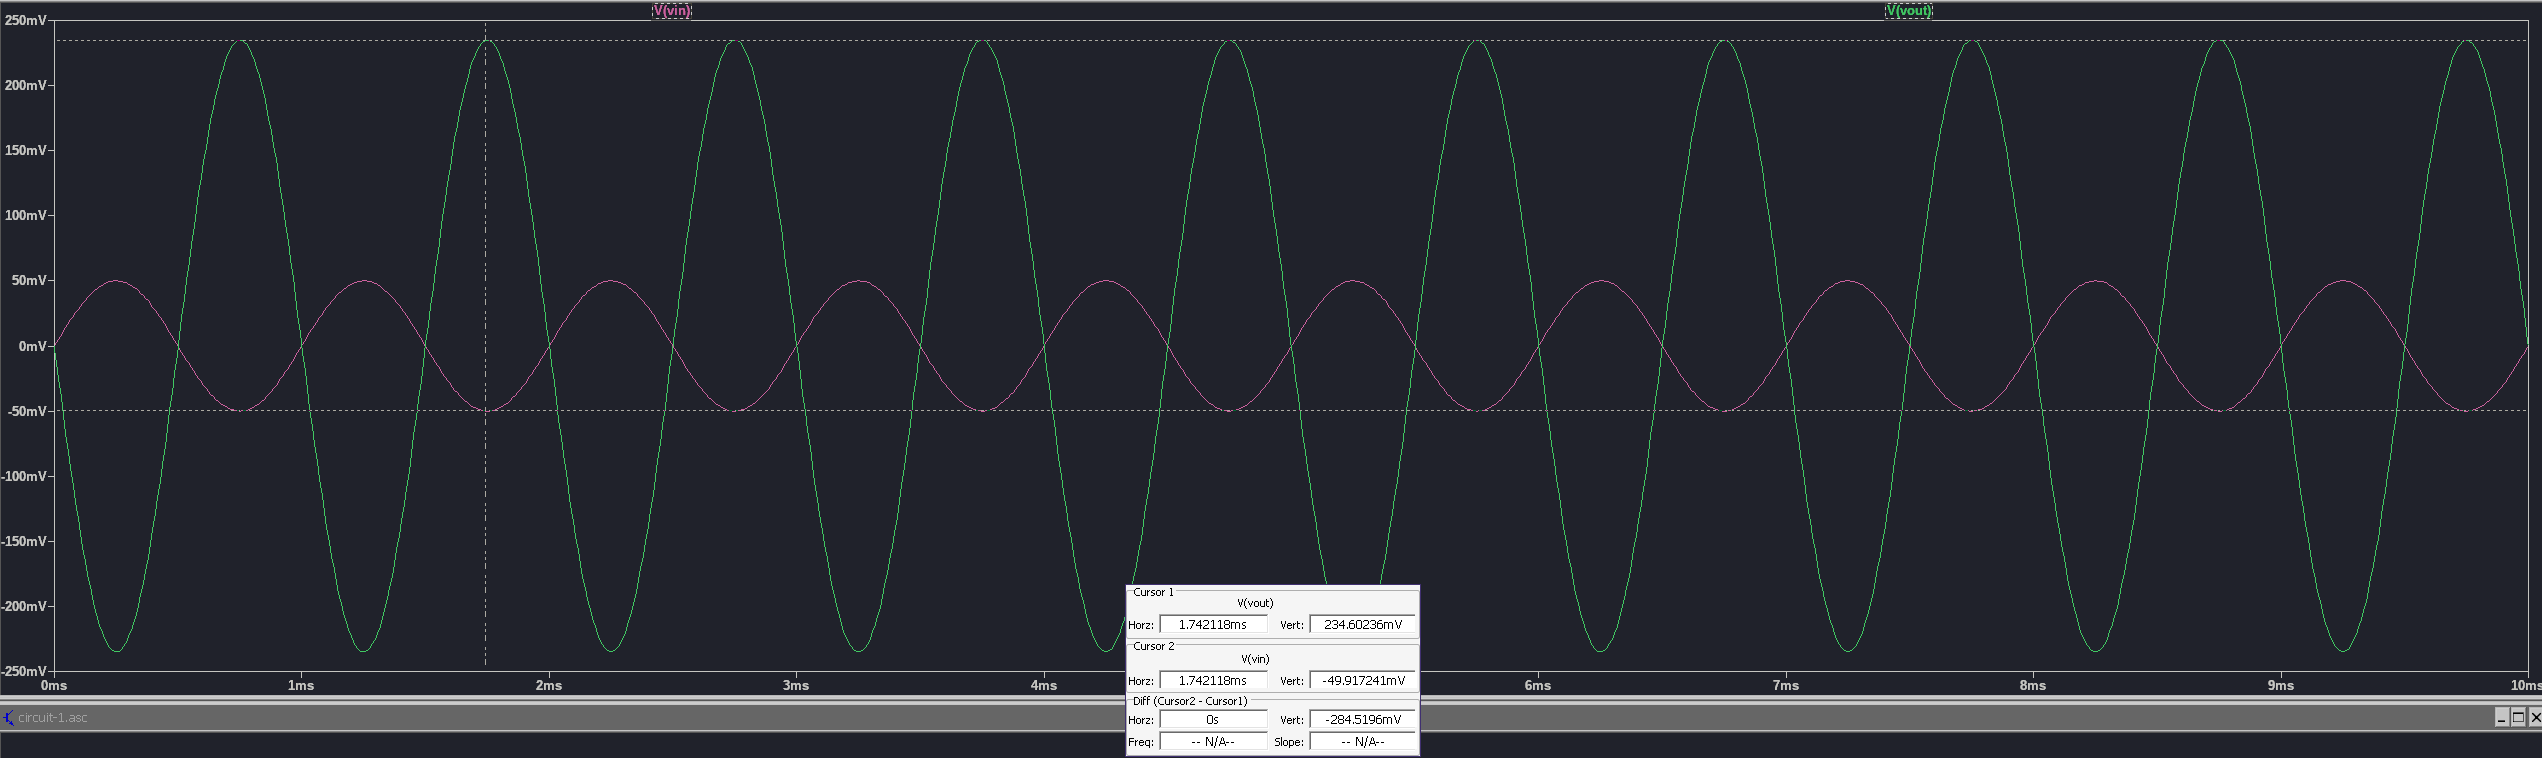
\includegraphics[width=\textwidth]{./assets/c1-trace.png}
	\caption{Circuit 1 Transient Simulation wtih Trace in LTspice}
	\label{fig:lts-c1-trace}
\end{figure}

The results given in Figure \ref{fig:lts-c1-trace} show a simulated input
voltage of -49.917 mV occuring at the same time as a simulated output voltage
of 234.602 mV; with some math, it can be found that simulated gain ratio is
-4.6998.

The non-inverting circuit was also simulated using LTSpice. The LTSpice circuit
schematic is shown in figure \ref{fig:lts-c2}.

\begin{figure}[H]
	\center
	
\includegraphics[width=\textwidth]{./assets/c2.png}
	\caption{Circuit 2 in LTspice}
	\label{fig:lts-c2}
\end{figure}

The schematic given by Figure \ref{fig:lts-c2} was used to run a transient
simulation, the results of which are given in Figure \ref{fig:lts-c2-trace}.

\begin{figure}[H]
	\center
	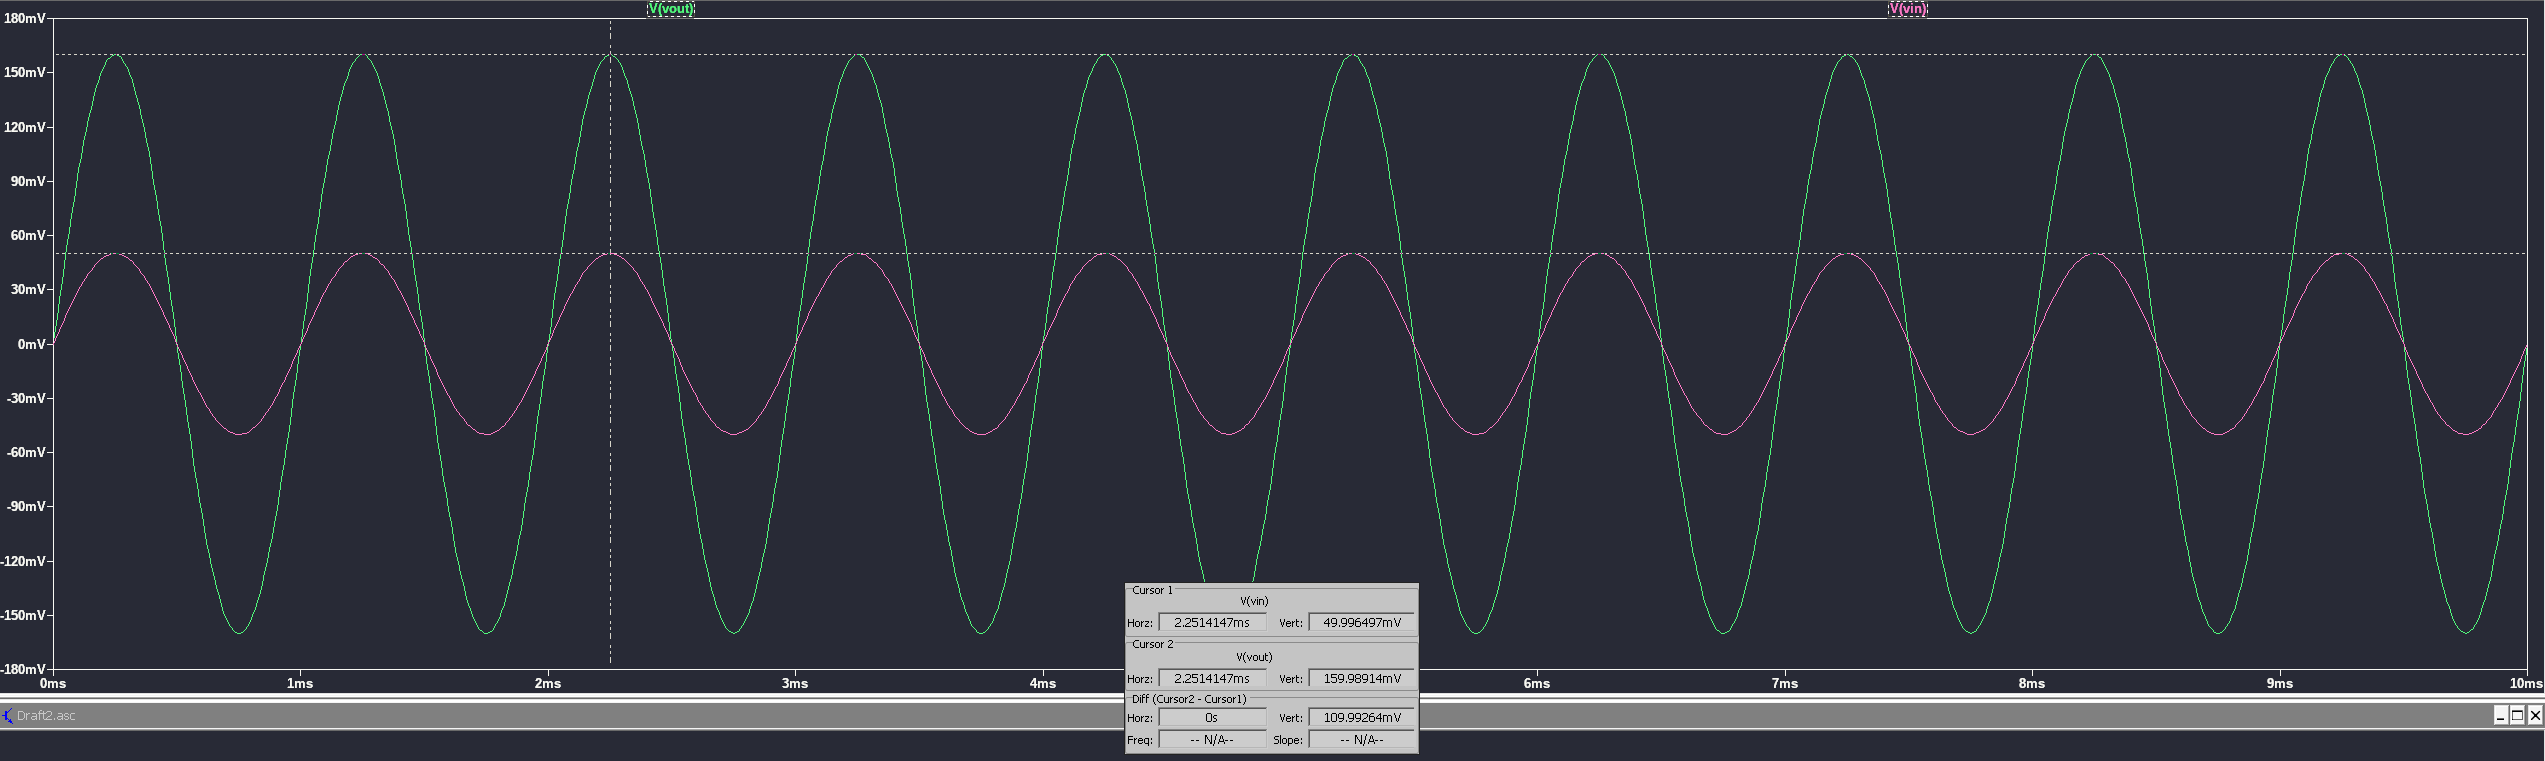
\includegraphics[width=\textwidth]{./assets/c2-trace.png}
	\caption{Circuit 2 Transient Simulation wtih Trace in LTspice}
	\label{fig:lts-c2-trace}
\end{figure}

The results given in Figure \ref{fig:lts-c2-trace} show a simulated input
voltage of 49.996 mV occuring at the same time as a simulated output voltage
of 159.9591 mV; with some math, it can be found that simulated gain ratio is
3.2000.

Simulation results were very similar to hand calculations; they differed by at
most 2 ten-thousandths of a millivolt.

\section{Hardware Experiment: Results and Discussion}

The inverting op-amp circuit given by Figure \ref{fig:lts-c1} was implemented
in hardware. The implementation is shown in Figure \ref{fig:c1-hw}.

\begin{figure}[H]
	\center
	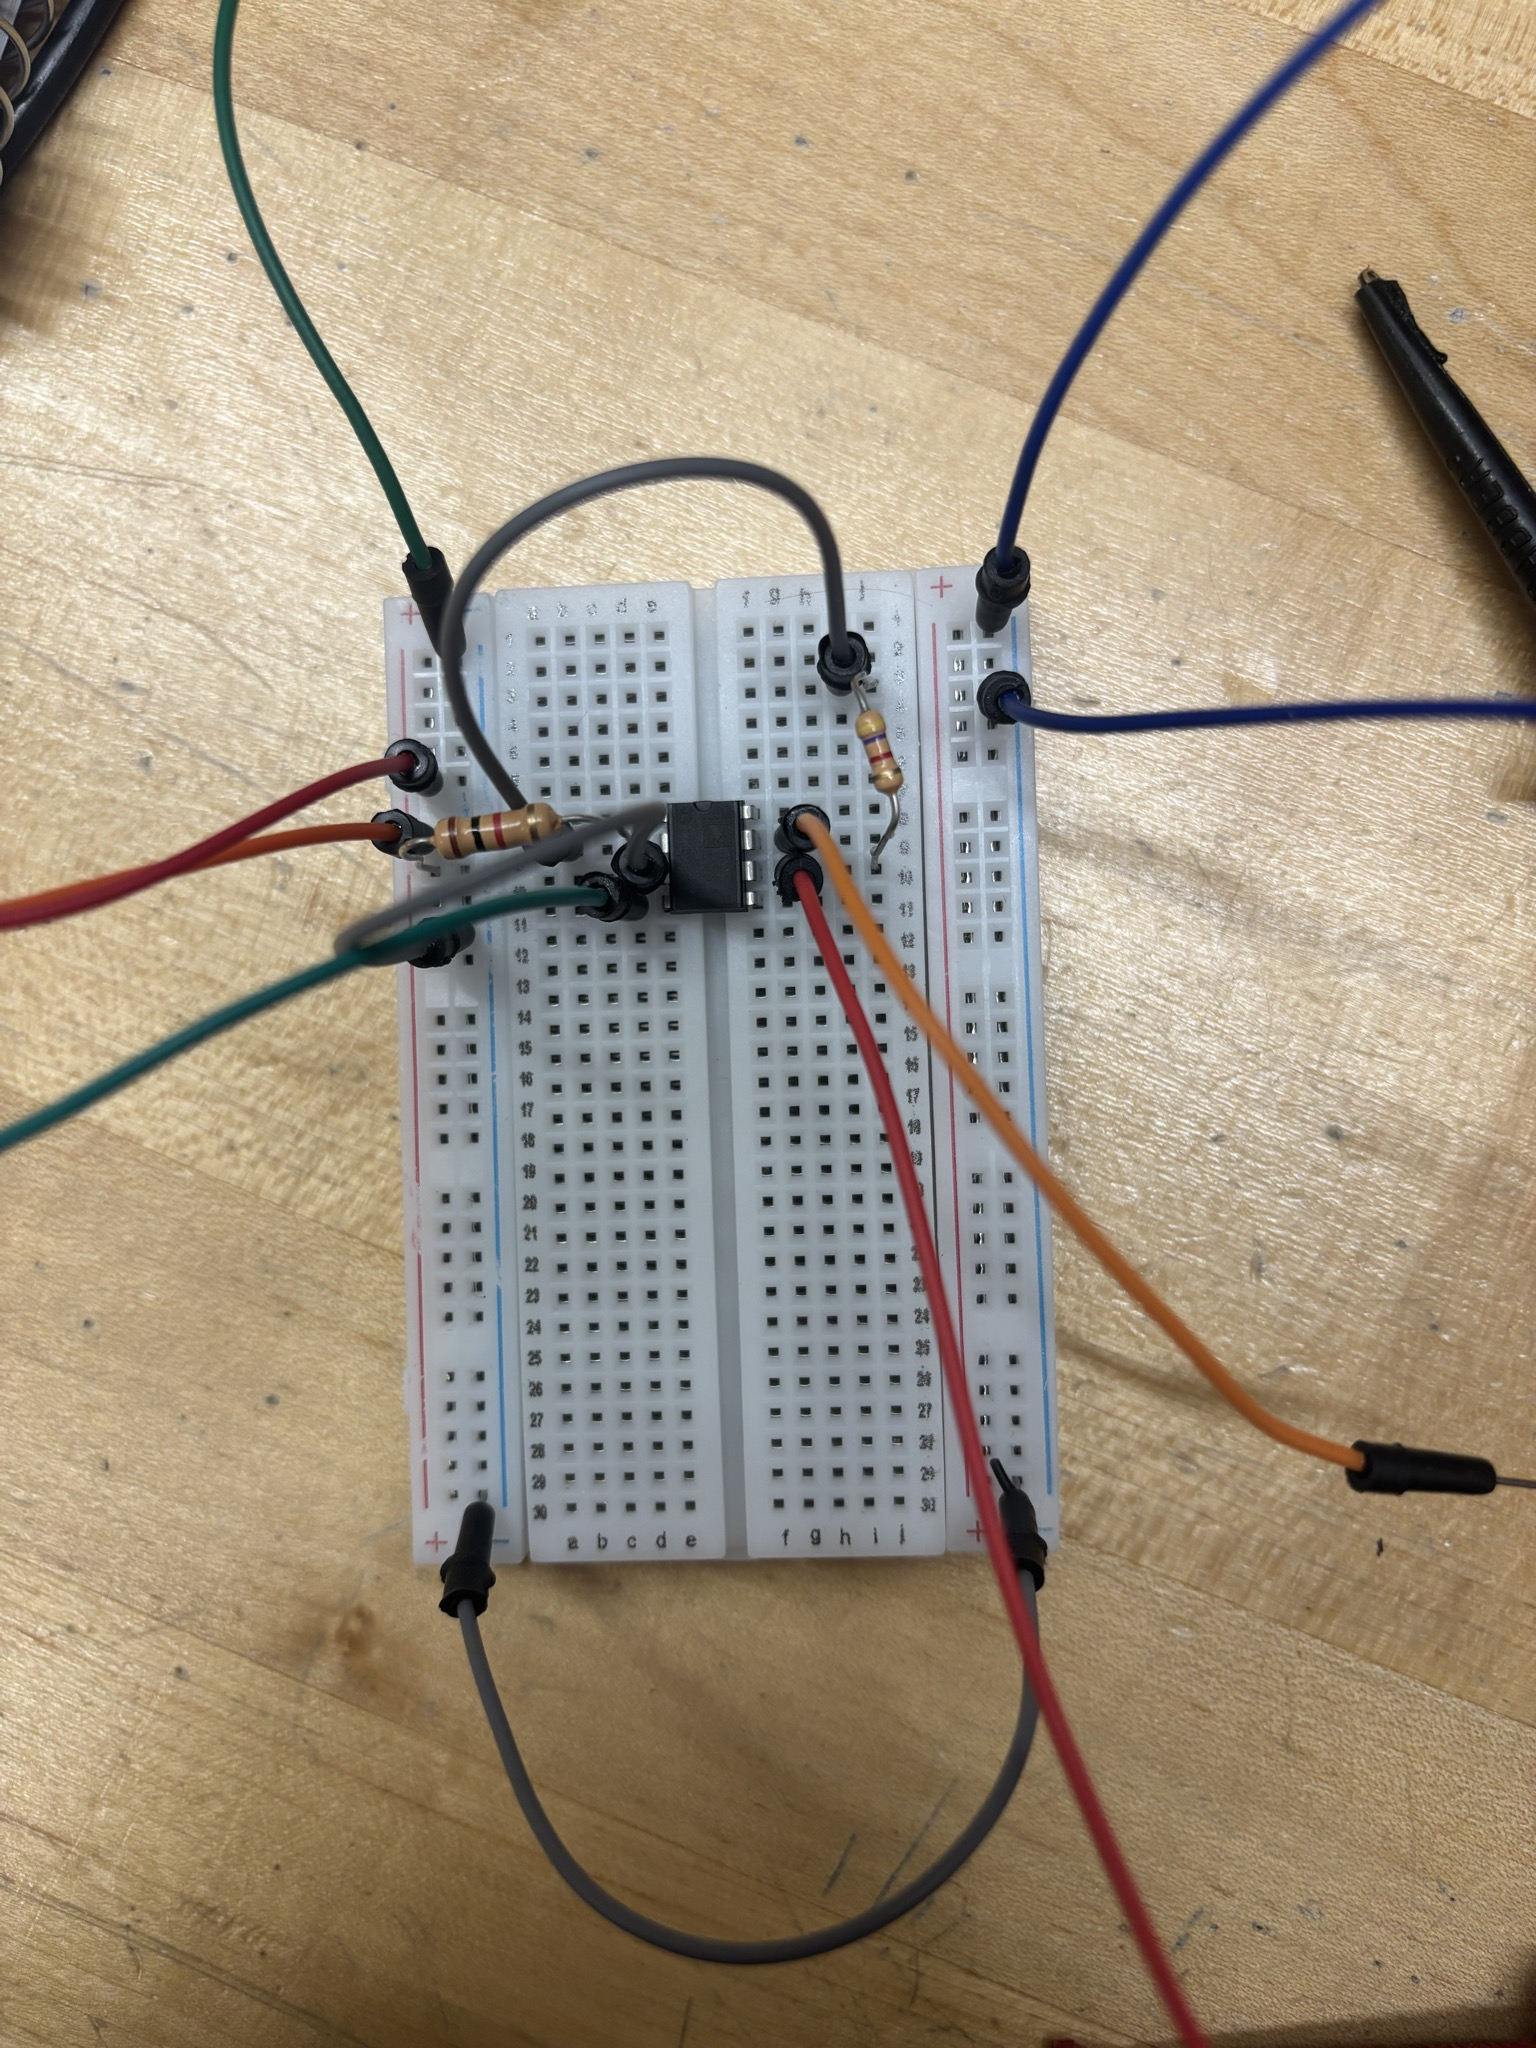
\includegraphics[width=0.5\textwidth]{./assets/c1-hw.jpg}
	\caption{Circuit 1 Hardware}
	\label{fig:c1-hw}
\end{figure}

The circuit was implemented on a breadboard. The center red wire (h10) and the
lower blue wire were used to connect the probes of an oscilliscope. A 1000 ohm
resistor was placed between the positive end of the voltage source and the
inverting terminal of the op amp.
A 4700 ohm resistor was placed between the inverting and output terminals
of the op amp. The oscilliscope reading is given in Figure \ref{fig:c1-osc}.

\begin{figure}[H]
	\center
	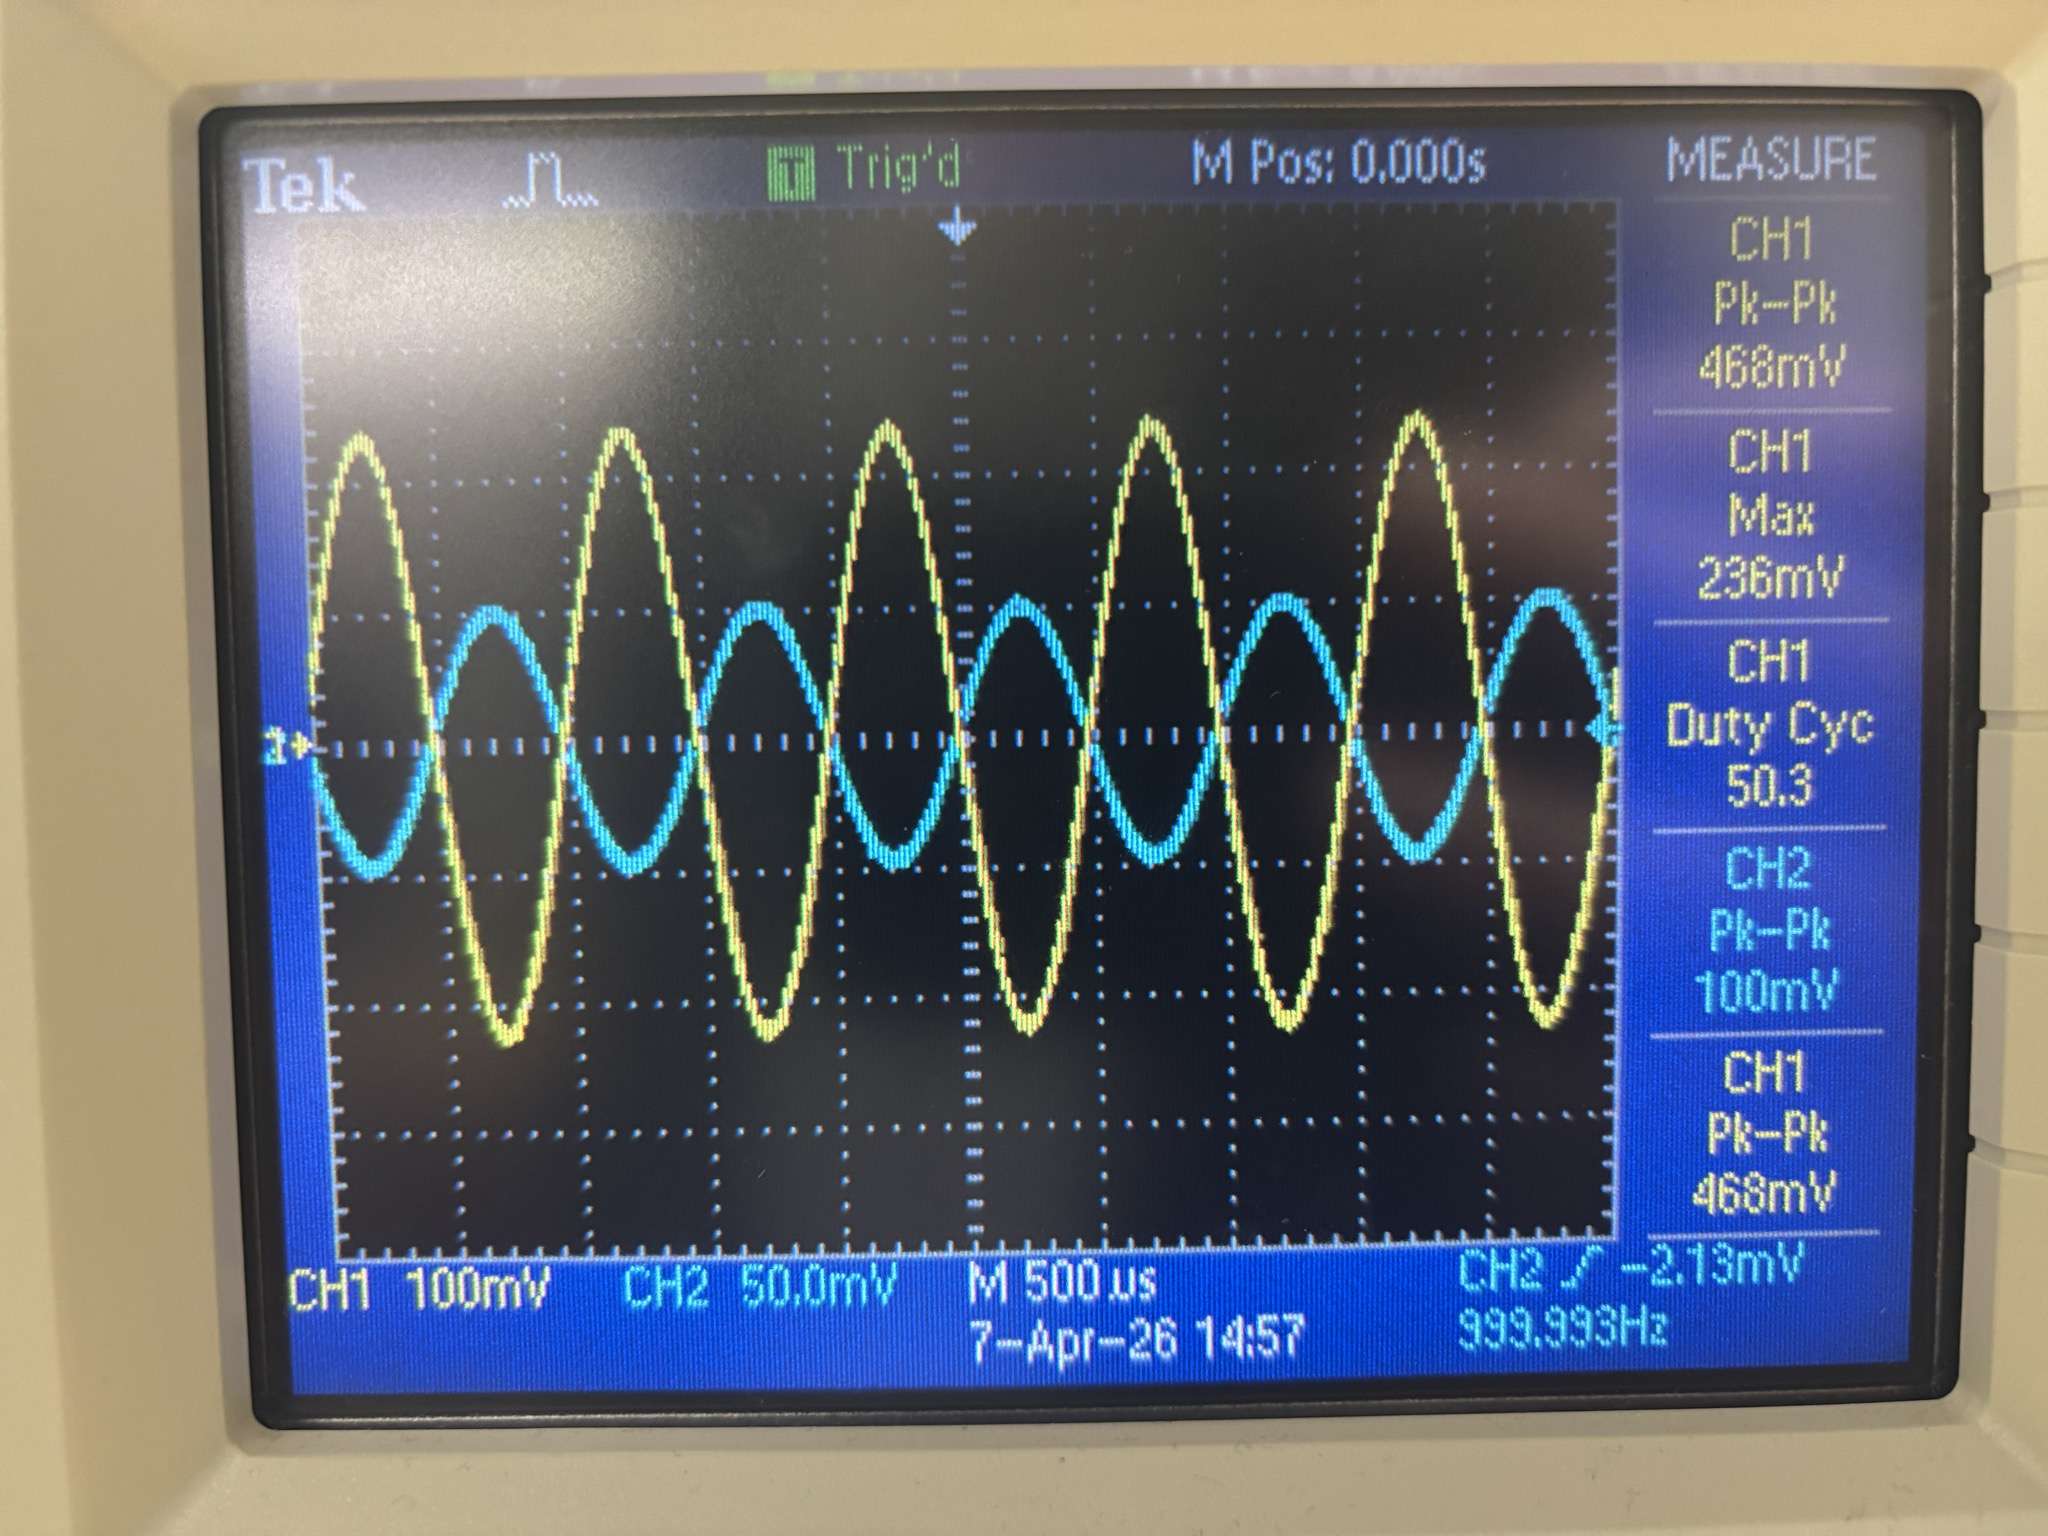
\includegraphics[width=0.5\textwidth]{./assets/c1-osc.jpg}
	\caption{Circuit 1 Oscilliscope Capture}
	\label{fig:c1-osc}
\end{figure}

The oscilliscope reading given in Figure \ref{fig:c1-osc} shows an output
peak-to-peak distance of 468 mV, compared to an input peak-to-peak distance of
100 mV. The waves are cleary out of phase by 180 degrees; the gain is negative.
The result is given in Table \ref{tab:hw}.

The non-inverting op-amp circuit given by Figure \ref{fig:lts-c2} was
implemented in hardware. The implementation is shown in Figure \ref{fig:c2-hw}.

\begin{figure}[H]
	\center
	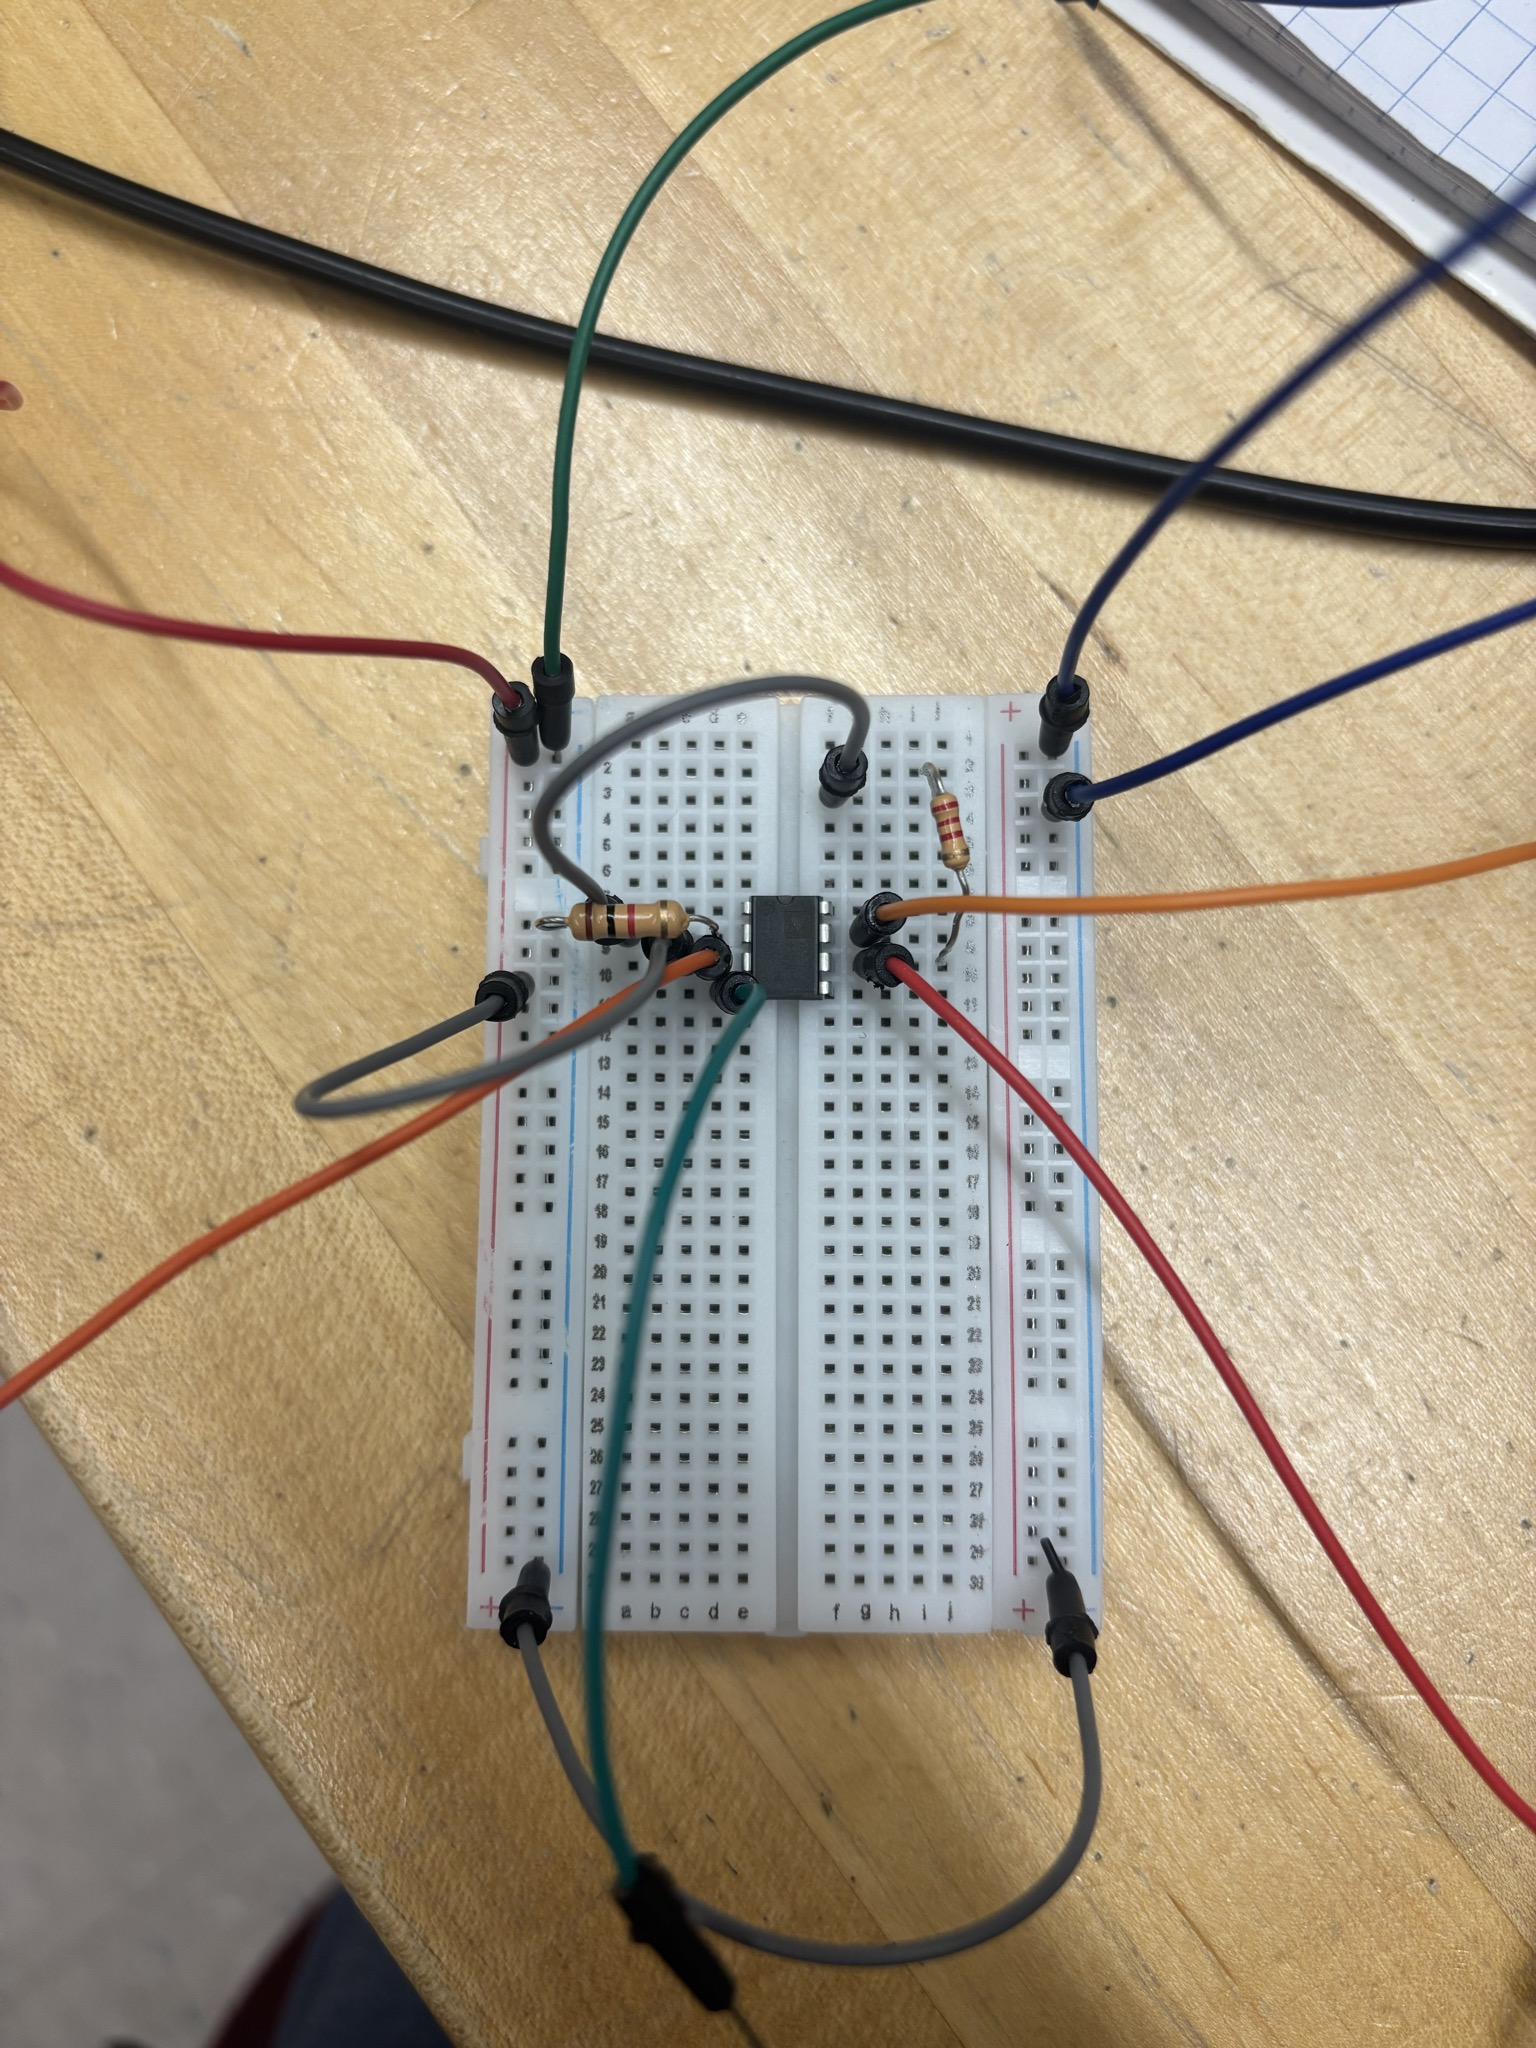
\includegraphics[width=0.5\textwidth]{./assets/c2-hw.jpg}
	\caption{Circuit 2 Hardware}
	\label{fig:c2-hw}
\end{figure}

The circuit was implemented on a breadboard. The center red wire (h10) and the
lower blue wire were used to connect the probes of an oscilliscope. A 1000 ohm
resistor was placed between ground and the inverting terminal of the op
amp. A 2200 ohm resistor was placed between the inverting and output terminals
of the op amp. The oscilliscope reading is given in Figure \ref{fig:c2-osc}.

\begin{figure}[H]
	\center
	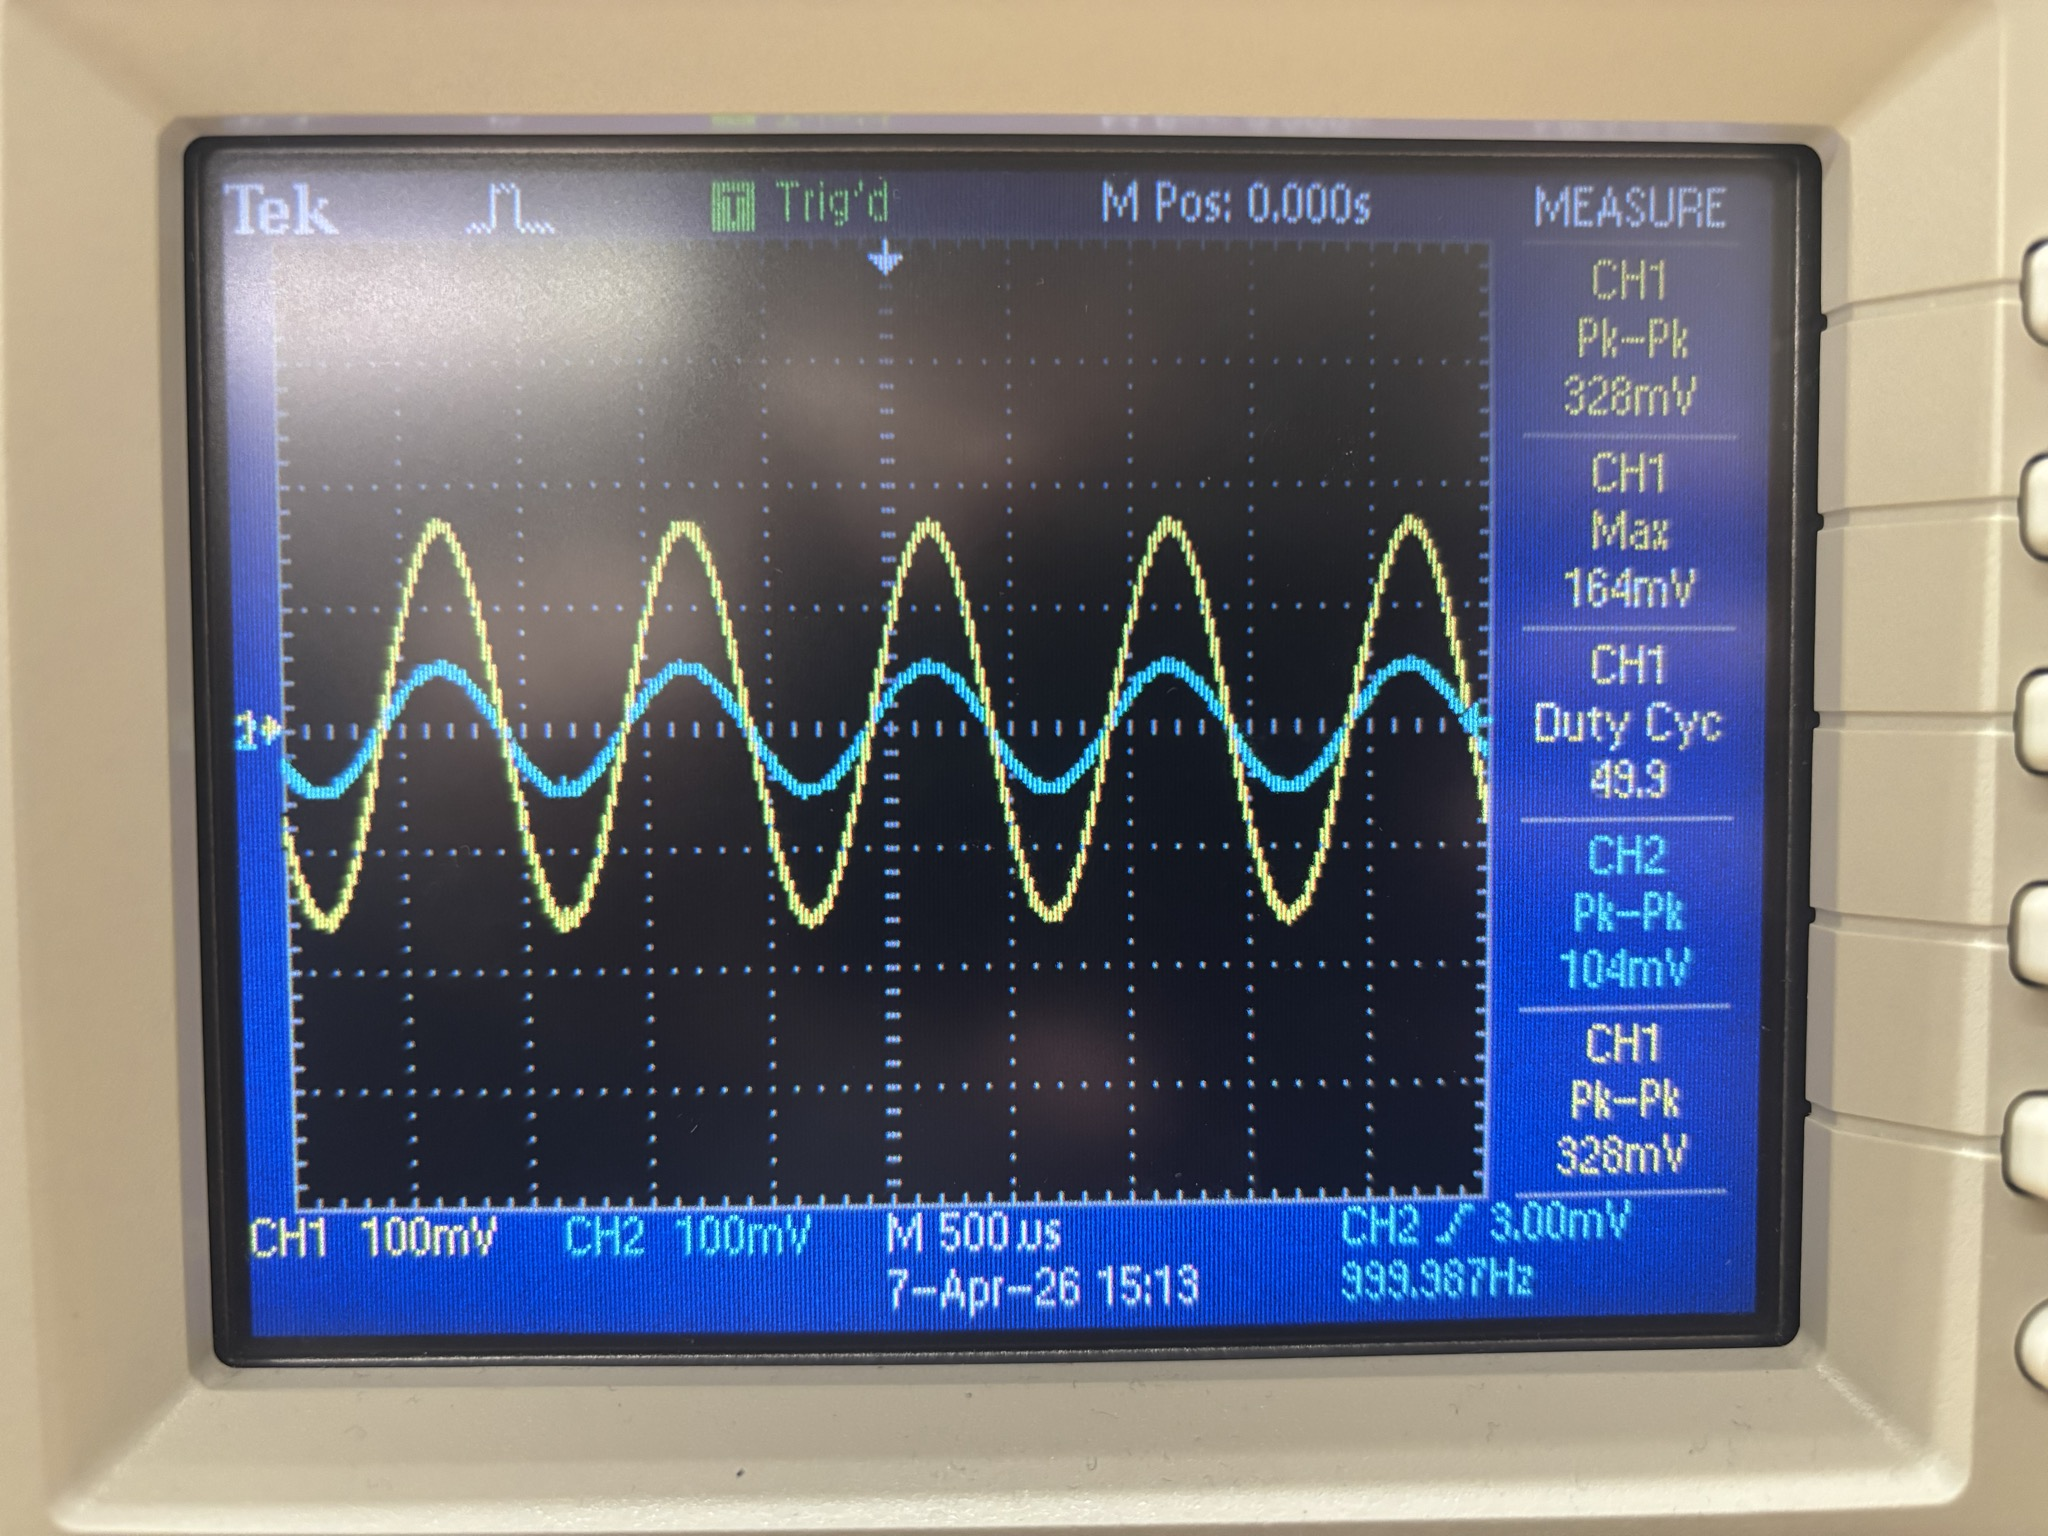
\includegraphics[width=0.5\textwidth]{./assets/c2-osc.jpg}
	\caption{Circuit 2 Oscilliscope Capture}
	\label{fig:c2-osc}
\end{figure}

The oscilliscope reading given in Figure \ref{fig:c2-osc} shows an output
peak-to-peak distance of 328 mV, compared to an input peak-to-peak distance of
104 mV. The waves are cleary in phase; the gain is positive. The result is
given in Table \ref{tab:hw}.

\begin{table}[H]
	\center
	\caption{Hardware Implementation Results}
	\begin{tabular}{|c||c|c|}
		\hline
		      & Inverting & Non-Inverting \\
		\hline
		\hline
		Gain  & -4.68     & 3.1538        \\
		\hline
		Error & -0.43\%   & -1.44\%       \\
		\hline
	\end{tabular}
	\label{tab:hw}
\end{table}

Table \ref{tab:hw} displays no significant error; both measurements are well
below 5\% error. The results are reasonable, based on previous simulations and
calculations.

\section{Conclusion}

All results are given in Table \ref{tab:res}.

\begin{table}[H]
	\center
	\caption{Final Laboratory Results}
	\begin{tabular}{|r|c|c|}
		\hline
		Label                      & Value   & Unit   \\
		\hline
		\hline
		$R_{\text{F.INV}}$         & 4700    & \Omega \\
		\hline
		$R_{\text{F.NON\_INV}}$    & 2200    & \Omega \\
		\hline
		LTspice Inverted Gain      & -4.6998 &        \\
		\hline
		LTspice Non-inverted Gain  & 3.2000  &        \\
		\hline
		Hardware Inverted Gain     & -4.6780 &        \\
		\hline
		Hardware Non-inverted Gain & 3.1538  &        \\
		\hline
	\end{tabular}
    \label{tab:res}
\end{table}

Circuit analysis techniques were used to determine the resistances required to
obtain an arbitrary gain ratio using both inverting and non-inverting
operational amplifiers. The calculated and simulated values were well within
acceptable error tolerances. This exercise was successful.

\section{Acknowledgements}

Methods described inthe the textbook \textit{Fundamentals of Electric Circuits,
	7th Edition} \cite{fec} were considered to find Thevenin equivalents.

The template for this Technical Memo was modified from a \LaTeX \ class created
by Joshua Milas and Seth Gower, using the provided Tech Memo Template and
example Tech Memo from the Advanced Course as inspiration.

The Teaching Assistant, Sol Holston, verified that calculated, simulated, and
measured values were correct.

\printbibliography

\end{document}
